% Options for packages loaded elsewhere
\PassOptionsToPackage{unicode}{hyperref}
\PassOptionsToPackage{hyphens}{url}
%
\documentclass[
]{article}
\usepackage{amsmath,amssymb}
\usepackage{lmodern}
\usepackage{iftex}
\ifPDFTeX
  \usepackage[T1]{fontenc}
  \usepackage[utf8]{inputenc}
  \usepackage{textcomp} % provide euro and other symbols
\else % if luatex or xetex
  \usepackage{unicode-math}
  \defaultfontfeatures{Scale=MatchLowercase}
  \defaultfontfeatures[\rmfamily]{Ligatures=TeX,Scale=1}
\fi
% Use upquote if available, for straight quotes in verbatim environments
\IfFileExists{upquote.sty}{\usepackage{upquote}}{}
\IfFileExists{microtype.sty}{% use microtype if available
  \usepackage[]{microtype}
  \UseMicrotypeSet[protrusion]{basicmath} % disable protrusion for tt fonts
}{}
\makeatletter
\@ifundefined{KOMAClassName}{% if non-KOMA class
  \IfFileExists{parskip.sty}{%
    \usepackage{parskip}
  }{% else
    \setlength{\parindent}{0pt}
    \setlength{\parskip}{6pt plus 2pt minus 1pt}}
}{% if KOMA class
  \KOMAoptions{parskip=half}}
\makeatother
\usepackage{xcolor}
\usepackage[margin=1in]{geometry}
\usepackage{color}
\usepackage{fancyvrb}
\newcommand{\VerbBar}{|}
\newcommand{\VERB}{\Verb[commandchars=\\\{\}]}
\DefineVerbatimEnvironment{Highlighting}{Verbatim}{commandchars=\\\{\}}
% Add ',fontsize=\small' for more characters per line
\usepackage{framed}
\definecolor{shadecolor}{RGB}{248,248,248}
\newenvironment{Shaded}{\begin{snugshade}}{\end{snugshade}}
\newcommand{\AlertTok}[1]{\textcolor[rgb]{0.94,0.16,0.16}{#1}}
\newcommand{\AnnotationTok}[1]{\textcolor[rgb]{0.56,0.35,0.01}{\textbf{\textit{#1}}}}
\newcommand{\AttributeTok}[1]{\textcolor[rgb]{0.77,0.63,0.00}{#1}}
\newcommand{\BaseNTok}[1]{\textcolor[rgb]{0.00,0.00,0.81}{#1}}
\newcommand{\BuiltInTok}[1]{#1}
\newcommand{\CharTok}[1]{\textcolor[rgb]{0.31,0.60,0.02}{#1}}
\newcommand{\CommentTok}[1]{\textcolor[rgb]{0.56,0.35,0.01}{\textit{#1}}}
\newcommand{\CommentVarTok}[1]{\textcolor[rgb]{0.56,0.35,0.01}{\textbf{\textit{#1}}}}
\newcommand{\ConstantTok}[1]{\textcolor[rgb]{0.00,0.00,0.00}{#1}}
\newcommand{\ControlFlowTok}[1]{\textcolor[rgb]{0.13,0.29,0.53}{\textbf{#1}}}
\newcommand{\DataTypeTok}[1]{\textcolor[rgb]{0.13,0.29,0.53}{#1}}
\newcommand{\DecValTok}[1]{\textcolor[rgb]{0.00,0.00,0.81}{#1}}
\newcommand{\DocumentationTok}[1]{\textcolor[rgb]{0.56,0.35,0.01}{\textbf{\textit{#1}}}}
\newcommand{\ErrorTok}[1]{\textcolor[rgb]{0.64,0.00,0.00}{\textbf{#1}}}
\newcommand{\ExtensionTok}[1]{#1}
\newcommand{\FloatTok}[1]{\textcolor[rgb]{0.00,0.00,0.81}{#1}}
\newcommand{\FunctionTok}[1]{\textcolor[rgb]{0.00,0.00,0.00}{#1}}
\newcommand{\ImportTok}[1]{#1}
\newcommand{\InformationTok}[1]{\textcolor[rgb]{0.56,0.35,0.01}{\textbf{\textit{#1}}}}
\newcommand{\KeywordTok}[1]{\textcolor[rgb]{0.13,0.29,0.53}{\textbf{#1}}}
\newcommand{\NormalTok}[1]{#1}
\newcommand{\OperatorTok}[1]{\textcolor[rgb]{0.81,0.36,0.00}{\textbf{#1}}}
\newcommand{\OtherTok}[1]{\textcolor[rgb]{0.56,0.35,0.01}{#1}}
\newcommand{\PreprocessorTok}[1]{\textcolor[rgb]{0.56,0.35,0.01}{\textit{#1}}}
\newcommand{\RegionMarkerTok}[1]{#1}
\newcommand{\SpecialCharTok}[1]{\textcolor[rgb]{0.00,0.00,0.00}{#1}}
\newcommand{\SpecialStringTok}[1]{\textcolor[rgb]{0.31,0.60,0.02}{#1}}
\newcommand{\StringTok}[1]{\textcolor[rgb]{0.31,0.60,0.02}{#1}}
\newcommand{\VariableTok}[1]{\textcolor[rgb]{0.00,0.00,0.00}{#1}}
\newcommand{\VerbatimStringTok}[1]{\textcolor[rgb]{0.31,0.60,0.02}{#1}}
\newcommand{\WarningTok}[1]{\textcolor[rgb]{0.56,0.35,0.01}{\textbf{\textit{#1}}}}
\usepackage{graphicx}
\makeatletter
\def\maxwidth{\ifdim\Gin@nat@width>\linewidth\linewidth\else\Gin@nat@width\fi}
\def\maxheight{\ifdim\Gin@nat@height>\textheight\textheight\else\Gin@nat@height\fi}
\makeatother
% Scale images if necessary, so that they will not overflow the page
% margins by default, and it is still possible to overwrite the defaults
% using explicit options in \includegraphics[width, height, ...]{}
\setkeys{Gin}{width=\maxwidth,height=\maxheight,keepaspectratio}
% Set default figure placement to htbp
\makeatletter
\def\fps@figure{htbp}
\makeatother
\setlength{\emergencystretch}{3em} % prevent overfull lines
\providecommand{\tightlist}{%
  \setlength{\itemsep}{0pt}\setlength{\parskip}{0pt}}
\setcounter{secnumdepth}{-\maxdimen} % remove section numbering
\ifLuaTeX
  \usepackage{selnolig}  % disable illegal ligatures
\fi
\IfFileExists{bookmark.sty}{\usepackage{bookmark}}{\usepackage{hyperref}}
\IfFileExists{xurl.sty}{\usepackage{xurl}}{} % add URL line breaks if available
\urlstyle{same} % disable monospaced font for URLs
\hypersetup{
  pdftitle={Thesis Figures and Code Snippets},
  pdfauthor={Samuel Richards},
  hidelinks,
  pdfcreator={LaTeX via pandoc}}

\title{Thesis Figures and Code Snippets}
\usepackage{etoolbox}
\makeatletter
\providecommand{\subtitle}[1]{% add subtitle to \maketitle
  \apptocmd{\@title}{\par {\large #1 \par}}{}{}
}
\makeatother
\subtitle{STA 610}
\author{Samuel Richards}
\date{}

\begin{document}
\maketitle

\hypertarget{artificial-neural-networks}{%
\section{Artificial Neural Networks}\label{artificial-neural-networks}}

\hypertarget{step-function}{%
\subsection{Step Function}\label{step-function}}

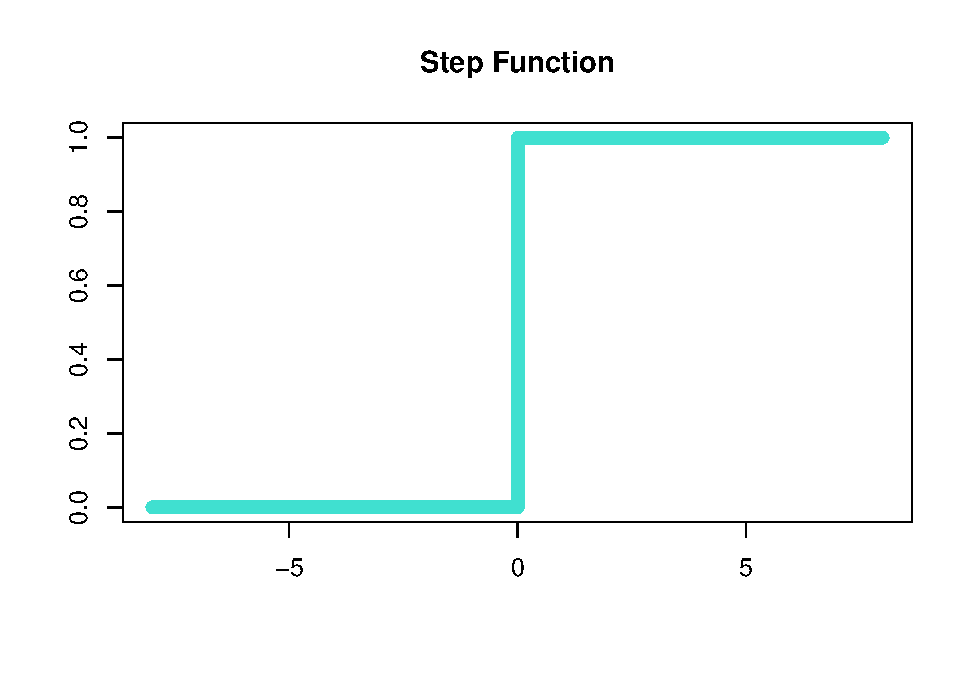
\includegraphics{Figures/step-function-1.pdf}

\hypertarget{sigmid-function}{%
\subsection{Sigmid Function}\label{sigmid-function}}

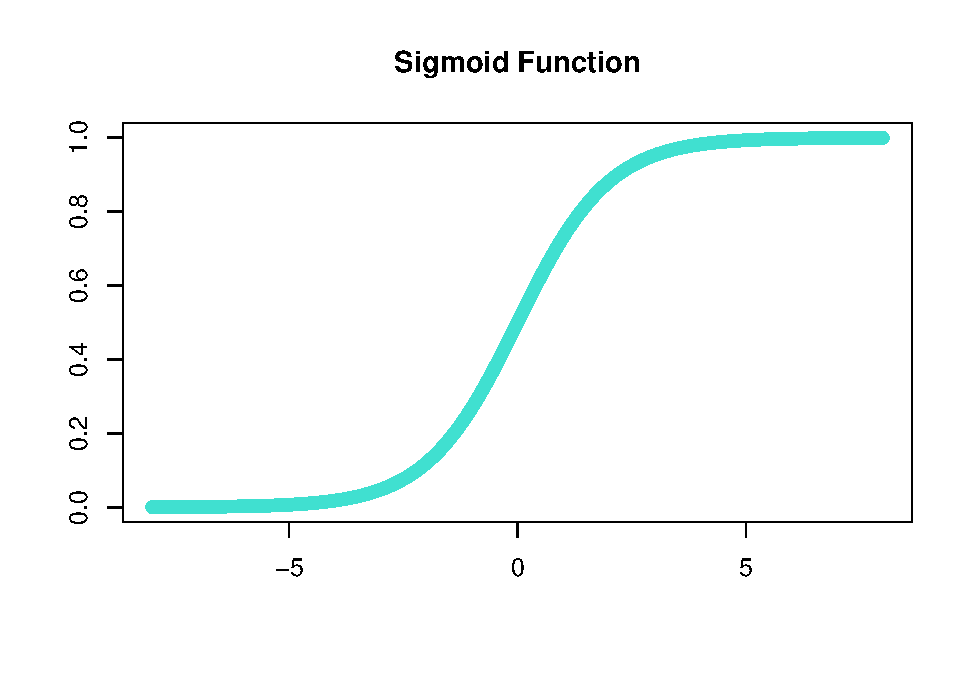
\includegraphics{Figures/sigmoid-function-1.pdf}

\hypertarget{other-activation-functions}{%
\subsection{Other Activation
Functions}\label{other-activation-functions}}

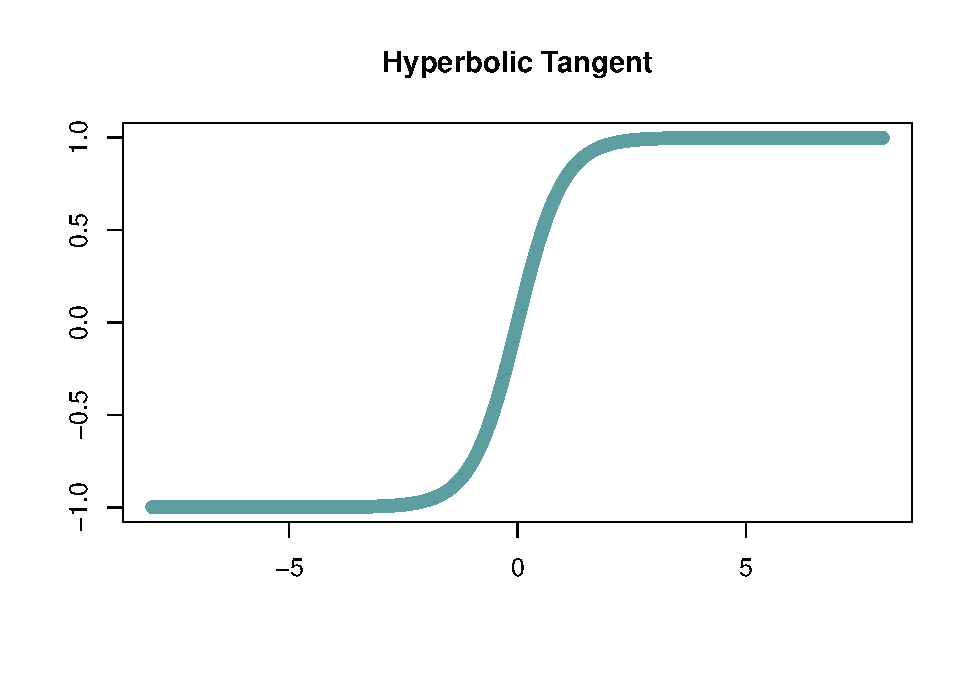
\includegraphics{Figures/other-activation-functions-1.pdf}
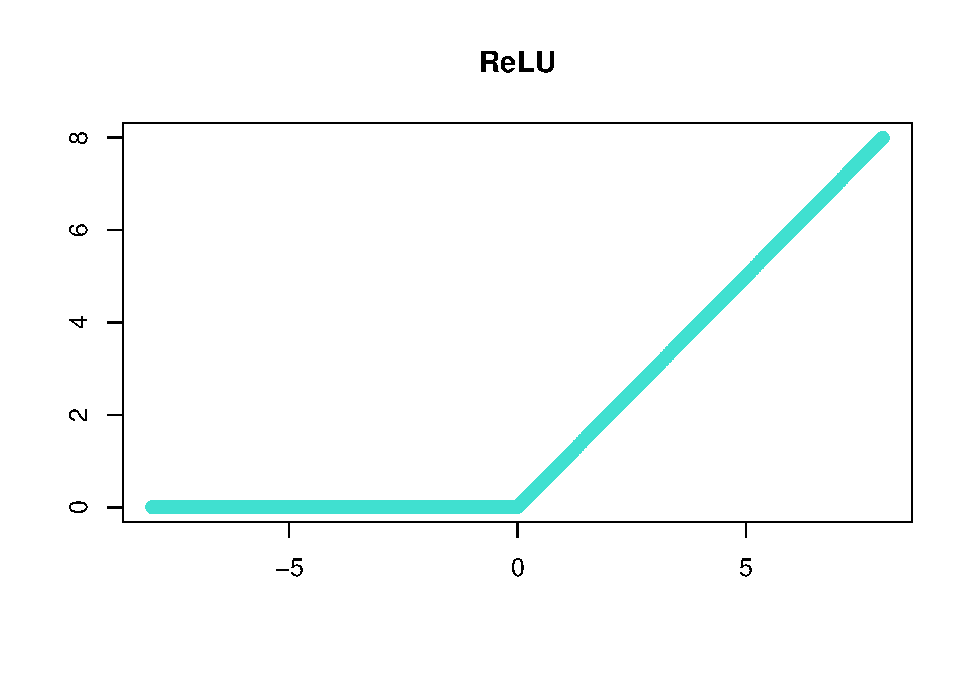
\includegraphics{Figures/other-activation-functions-2.pdf}

\hypertarget{gradient-descent}{%
\subsection{Gradient Descent}\label{gradient-descent}}

\hypertarget{d-example}{%
\subsubsection{2-D example}\label{d-example}}

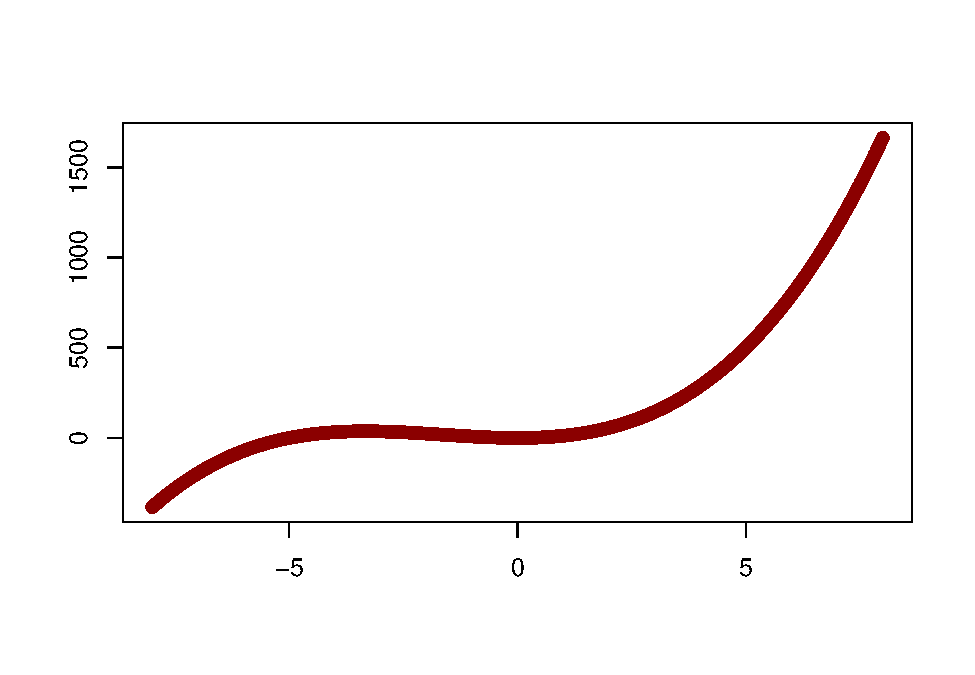
\includegraphics{Figures/grad_desc_2D-1.pdf}

\hypertarget{d-example-1}{%
\subsubsection{3-D example}\label{d-example-1}}

\hypertarget{regularization}{%
\subsection{Regularization}\label{regularization}}

\hypertarget{overfit-and-underfit}{%
\subsubsection{Overfit and Underfit}\label{overfit-and-underfit}}

\begin{Shaded}
\begin{Highlighting}[]
\CommentTok{\#Generate some noisy data}
\FunctionTok{set.seed}\NormalTok{(}\DecValTok{3}\NormalTok{)}
\NormalTok{a }\OtherTok{\textless{}{-}} \FunctionTok{runif}\NormalTok{(}\DecValTok{12}\NormalTok{, }\AttributeTok{min=}\DecValTok{0}\NormalTok{, }\AttributeTok{max=}\DecValTok{90}\NormalTok{)}
\NormalTok{c }\OtherTok{\textless{}{-}} \DecValTok{24}\SpecialCharTok{*}\FunctionTok{sin}\NormalTok{(.}\DecValTok{05}\SpecialCharTok{*}\NormalTok{a) }\SpecialCharTok{+} \FunctionTok{rnorm}\NormalTok{(}\FunctionTok{length}\NormalTok{(a),}\DecValTok{0}\NormalTok{,}\DecValTok{5}\NormalTok{) }\SpecialCharTok{+} \DecValTok{40}

\CommentTok{\#create data frame and base plot}
\NormalTok{df }\OtherTok{\textless{}{-}} \FunctionTok{data.frame}\NormalTok{(a,c)}
\NormalTok{model }\OtherTok{\textless{}{-}} \FunctionTok{ggplot}\NormalTok{(df, }\FunctionTok{aes}\NormalTok{(}\AttributeTok{x =}\NormalTok{ a, }\AttributeTok{y =}\NormalTok{ c)) }\SpecialCharTok{+}
        \FunctionTok{geom\_point}\NormalTok{(}\AttributeTok{size =} \DecValTok{3}\NormalTok{, }\AttributeTok{color =} \StringTok{"purple"}\NormalTok{) }\SpecialCharTok{+}
        \FunctionTok{ylim}\NormalTok{(}\DecValTok{30}\NormalTok{,}\DecValTok{80}\NormalTok{) }\SpecialCharTok{+}
        \FunctionTok{theme\_minimal}\NormalTok{()}


\CommentTok{\# underfit model}

\NormalTok{model }\SpecialCharTok{+}
    \FunctionTok{stat\_smooth}\NormalTok{(}\AttributeTok{method =}\NormalTok{ lm,}
              \AttributeTok{formula =}\NormalTok{ y }\SpecialCharTok{\textasciitilde{}} \FunctionTok{poly}\NormalTok{(x,}\DecValTok{1}\NormalTok{),}
              \AttributeTok{fullrange =}\NormalTok{ T,}
              \AttributeTok{color =} \StringTok{"turquoise"}\NormalTok{,}
              \AttributeTok{se =}\NormalTok{ F)}
\end{Highlighting}
\end{Shaded}

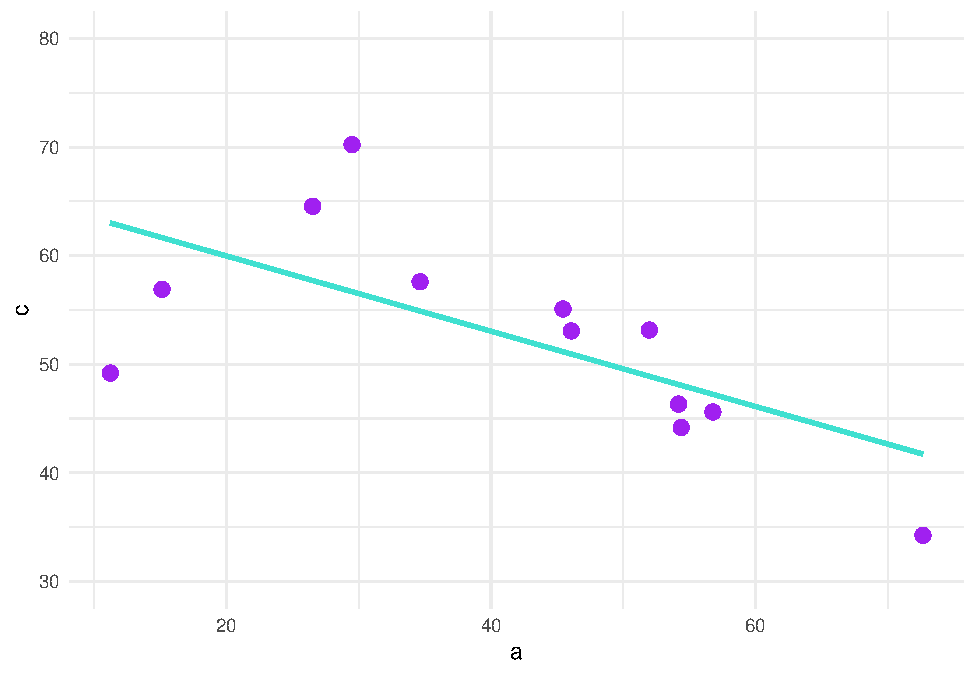
\includegraphics{Figures/unnamed-chunk-1-1.pdf}

\begin{Shaded}
\begin{Highlighting}[]
\CommentTok{\# overfit model}

\NormalTok{pol }\OtherTok{\textless{}{-}} \DecValTok{9} \CommentTok{\# polynomial order}
\NormalTok{model }\SpecialCharTok{+} 
    \FunctionTok{stat\_smooth}\NormalTok{(}\AttributeTok{method =}\NormalTok{ lm,}
              \AttributeTok{formula =}\NormalTok{ y }\SpecialCharTok{\textasciitilde{}} \FunctionTok{poly}\NormalTok{(x,pol),}
              \AttributeTok{fullrange =}\NormalTok{ T,}
              \AttributeTok{color =} \StringTok{"turquoise"}\NormalTok{,}
              \AttributeTok{se =}\NormalTok{ F)}
\end{Highlighting}
\end{Shaded}

\begin{verbatim}
## Warning: Removed 16 rows containing missing values (`geom_smooth()`).
\end{verbatim}

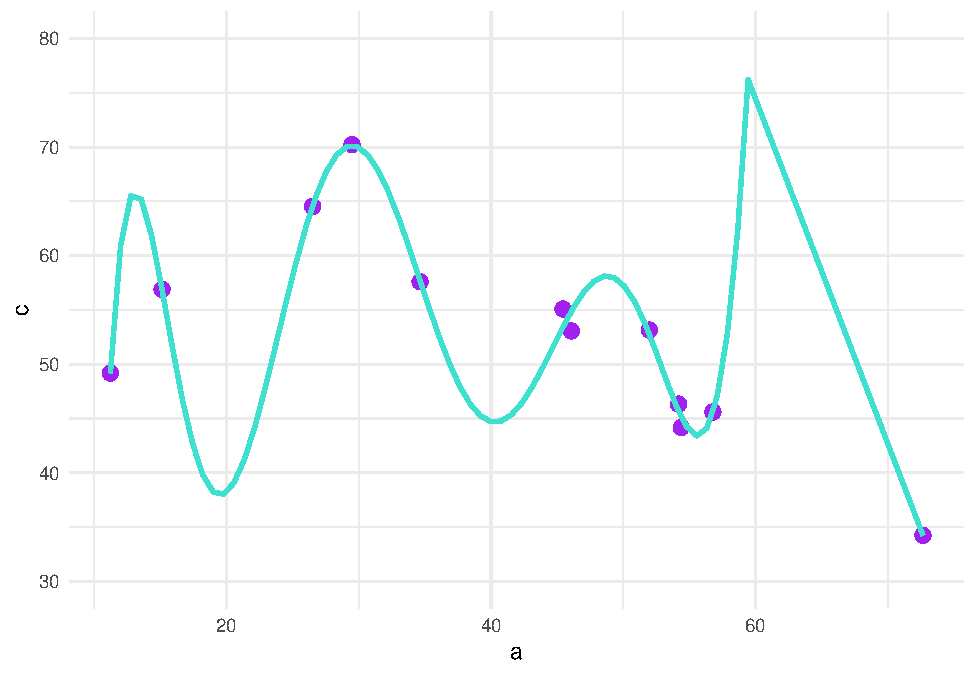
\includegraphics{Figures/unnamed-chunk-1-2.pdf}

\hypertarget{bayes}{%
\section{Bayes}\label{bayes}}

\hypertarget{bayesian-updating}{%
\subsection{Bayesian Updating}\label{bayesian-updating}}

For each possible explaination of the sample, count all the ways in
which the sample could happen. Explanations with more ways to produce
the sample are more plausible.

\begin{Shaded}
\begin{Highlighting}[]
\CommentTok{\#ways/sum(ways)}

\NormalTok{prob }\OtherTok{\textless{}{-}} \FunctionTok{runif}\NormalTok{(}\DecValTok{1}\NormalTok{,}\DecValTok{0}\NormalTok{,}\DecValTok{1}\NormalTok{) }\CommentTok{\#single observation from a uniform distribution to be the probability we want to find}


\NormalTok{sample }\OtherTok{\textless{}{-}} \FunctionTok{rbinom}\NormalTok{(}\DecValTok{100}\NormalTok{,}\DecValTok{1}\NormalTok{, prob)}
\CommentTok{\#plot(sample)}

\NormalTok{W }\OtherTok{\textless{}{-}} \FunctionTok{sum}\NormalTok{(sample}\SpecialCharTok{==}\StringTok{"1"}\NormalTok{)}
\NormalTok{L }\OtherTok{\textless{}{-}} \FunctionTok{sum}\NormalTok{(sample}\SpecialCharTok{==}\StringTok{"0"}\NormalTok{)}
\CommentTok{\#p \textless{}{-} seq(0,1,length = 100)}


\NormalTok{p\_grid }\OtherTok{\textless{}{-}} \FunctionTok{seq}\NormalTok{(}\AttributeTok{from=}\DecValTok{0}\NormalTok{, }\AttributeTok{to=}\DecValTok{1}\NormalTok{, }\AttributeTok{length.out =} \DecValTok{100}\NormalTok{)  }\CommentTok{\#100 values for proportion (p) between 0 and 1}

\CommentTok{\#prior distribution }
\NormalTok{prior }\OtherTok{\textless{}{-}} \FunctionTok{dbeta}\NormalTok{(p\_grid, }\DecValTok{10}\NormalTok{,}\DecValTok{10}\NormalTok{) }\CommentTok{\#(interval of previous assumptions/explanations (p) and the probability for each value)}

\CommentTok{\#(note that you do not need data for a prior distribution {-} the data washes out the "falsities" of the prior)}

\NormalTok{likelihood }\OtherTok{\textless{}{-}} \FunctionTok{dbinom}\NormalTok{(}\FunctionTok{sum}\NormalTok{(W), }\AttributeTok{size=}\DecValTok{100}\NormalTok{, }\AttributeTok{prob=}\NormalTok{p\_grid) }\CommentTok{\#Relative number of ways we can see W out of (W+L) from the Binomial Sampling Formula for all of the respective proportions outlined in p\_grid}

\NormalTok{posterior }\OtherTok{\textless{}{-}}\NormalTok{ likelihood }\SpecialCharTok{*}\NormalTok{ prior }\CommentTok{\#sets up and normalizes the posterior distribution}
\NormalTok{posterior }\OtherTok{\textless{}{-}}\NormalTok{ posterior }\SpecialCharTok{/} \FunctionTok{sum}\NormalTok{(posterior)}


\FunctionTok{plot}\NormalTok{(prior)}
\end{Highlighting}
\end{Shaded}

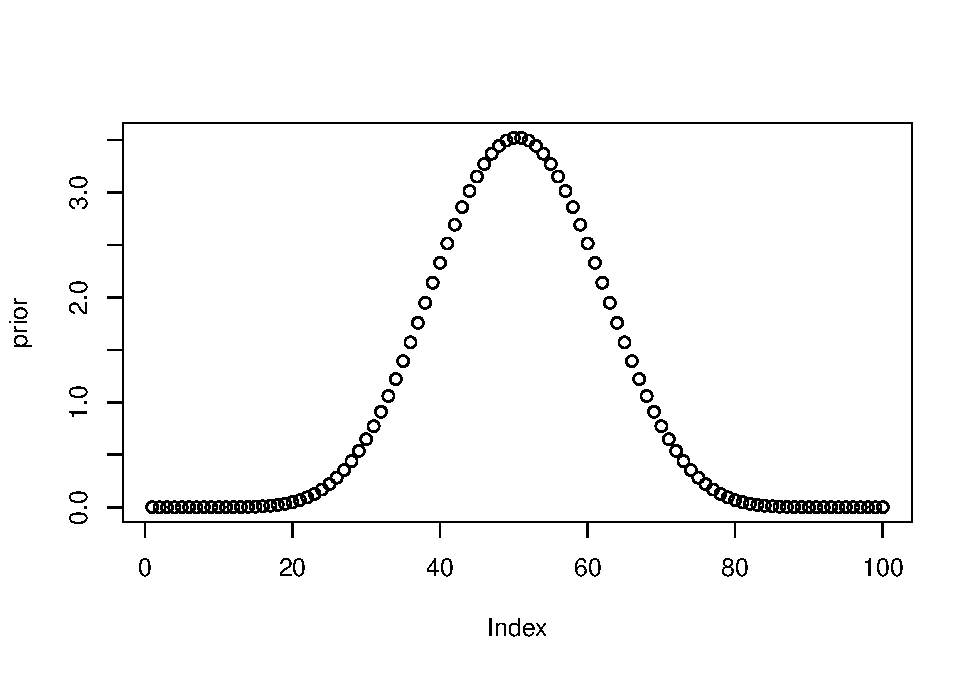
\includegraphics{Figures/unnamed-chunk-3-1.pdf}

\begin{Shaded}
\begin{Highlighting}[]
\FunctionTok{plot}\NormalTok{(likelihood)}
\end{Highlighting}
\end{Shaded}

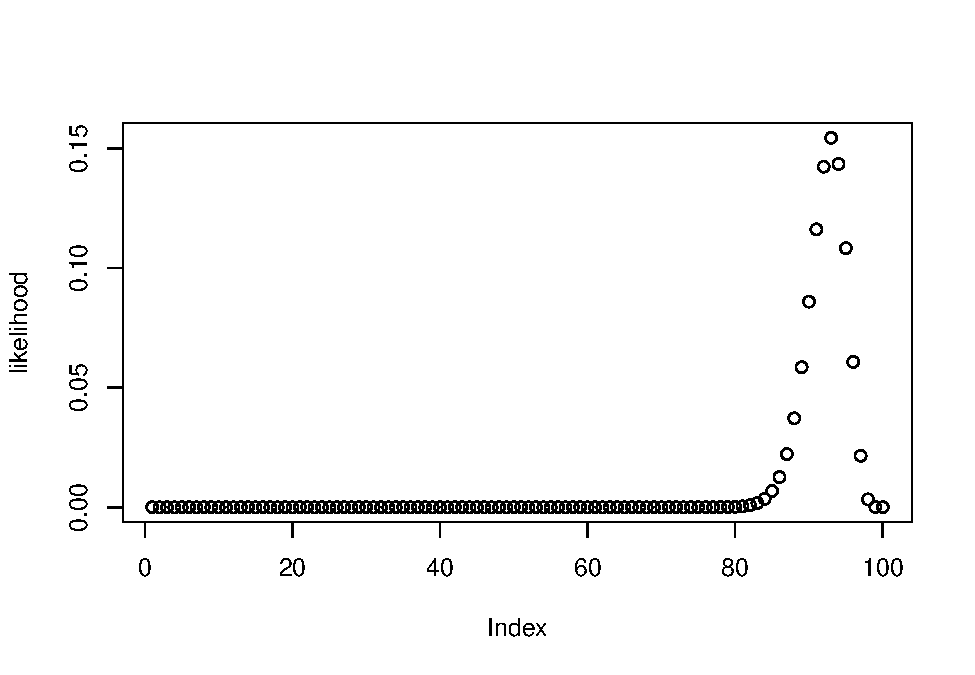
\includegraphics{Figures/unnamed-chunk-3-2.pdf}

\begin{Shaded}
\begin{Highlighting}[]
\FunctionTok{plot}\NormalTok{(posterior)    }\CommentTok{\#plots the posterior distribution}
\end{Highlighting}
\end{Shaded}

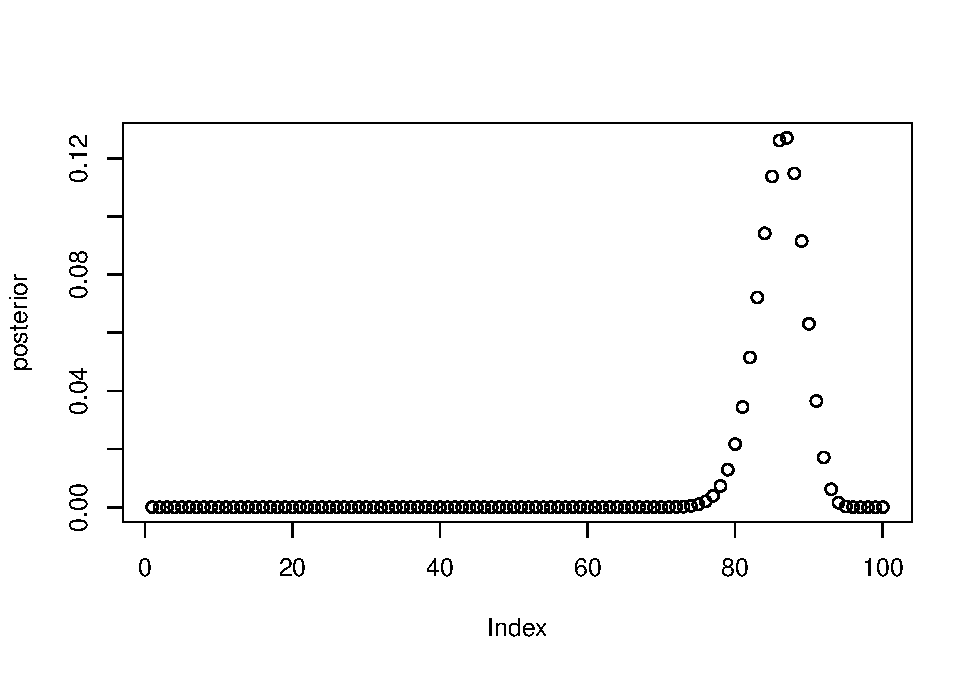
\includegraphics{Figures/unnamed-chunk-3-3.pdf}

\end{document}
